\documentclass[11pt,a4paper]{article}
\usepackage[utf8]{inputenc}
\usepackage[T1]{fontenc}
\usepackage{amsmath,amssymb,amsthm}
\usepackage{booktabs}
\usepackage{graphicx}
\usepackage{hyperref}
\usepackage{natbib}
\usepackage{geometry}
\geometry{a4paper, margin=1in}
\usepackage{setspace}
\usepackage{caption}
\usepackage{array}
\usepackage{multirow}
\usepackage{float}

\hypersetup{
    colorlinks=true,
    linkcolor=blue,
    citecolor=blue,
    urlcolor=blue,
    pdftitle={Directional Decoupling and the Volatility-Ratio Channel},
    pdfauthor={HoKwang Kim}
}

\title{\textbf{Directional Decoupling and the Volatility-Ratio Channel: \\
A Beta-Decomposition Framework for Exchange-Native Tokens \\[0.3em]
\large\normalfont\itshape Evidence from the BNB--ETH Relationship, 2022--2026}}

\author{
HoKwang Kim\thanks{CEO, Betalabs Inc., Seoul, South Korea. ORCID: \href{https://orcid.org/0009-0002-0962-2175}{0009-0002-0962-2175}. Email: \texttt{gameworker@gmail.com}. The author has worked in the blockchain industry since 2017, serving as a long-standing intermediary between the Korean and Chinese blockchain ecosystems with substantial contributions to mainnet infrastructure, exchange security, regulatory policy, and token-listing strategy. In 2022 he was appointed CEO and CTO of Cyworld---the world's first social network---where he led the recovery of 3.8 petabytes of historical user data and approximately 18 billion photographs. Replication code, datasets, and the working paper are available at \url{https://github.com/gameworkerkim/vibe-investing}. The author thanks anonymous reviewers and acknowledges that this is a working paper version. All errors are the author's own.} \\
\textit{Betalabs Inc.}
}

\date{May 2026 \\ \small Working Paper Version 9.2 (Final)}

\begin{document}

\maketitle
\onehalfspacing

\begin{abstract}
\noindent Standard factor models in cryptocurrency asset pricing \citep{liu2021,liu2024} treat beta as a sufficient statistic for systematic exposure. The identity $\beta = \rho \cdot (\sigma_i/\sigma_m)$ implies, however, that beta can change for two distinct reasons: a change in directional co-movement (correlation channel) or a change in relative volatility (volatility-ratio channel). The economic interpretations differ sharply, but the existing literature does not systematically separate them.

\textbf{This paper proposes a variance-decomposition framework that isolates the two channels}, and applies it to a striking empirical pattern in cryptocurrency markets that we term \textit{directional decoupling}: a beta decline accompanied by an unchanged correlation. Using daily price data from CoinMetrics covering May 2022 to April 2026 ($n=1{,}460$ trading days), we document that BNB's static beta to Ethereum (ETH) falls by 16.9\% (from 0.643 to 0.534) while the Pearson correlation remains essentially unchanged ($0.731 \to 0.731$). \textbf{The decomposition reveals that 100\% of the static beta change is attributable to a decline in the volatility ratio $\sigma_{BNB}/\sigma_{ETH}$ (from 0.879 to 0.730), with no contribution from correlation change.} A further numerator/denominator decomposition shows that BNB-side volatility compression accounts for approximately 57\% of the ratio decline, while ETH-side volatility expansion accounts for approximately 43\% --- indicating that the apparent BNB pattern is jointly produced by BNB-specific and ETH-side dynamics. DCC-GARCH \citep{engle2002} estimation confirms the qualitative pattern under dynamic conditional moments: dynamic correlation rises ($0.698 \to 0.747$, $p<0.001$) while dynamic beta declines ($0.575 \to 0.541$, $-5.84\%$).

Cross-sectional analysis of 16 altcoins (exchange tokens, Layer-1 platforms, DeFi/oracle, and other major altcoins) reveals substantial heterogeneity in beta dynamics across and within categories, with BNB occupying the moderate-to-strong decoupling segment but not an extreme position (BNB rank 6/17 in the cross-sectional pool, $t=-2.22$, $p=0.043$ against the control mean; synthetic-control rank 12/17, $p\approx 0.71$). The cross-sectional evidence supports interpreting BNB's pattern as part of a broader altcoin beta-recompression coinciding with ETH's volatility expansion post-2024, rather than as an asset-specific regime change. We discuss implications for cryptocurrency factor models---specifically, that beta-based models should be augmented with explicit decomposition into correlation and volatility-ratio components when interpreting systematic-exposure changes---and identify on-chain stablecoin flow data and staggered-treatment designs around individual exchange holder-reward launches as priority directions for follow-up causal-mechanism studies. The April 2024 launch of the Binance HODLer Airdrops program serves as a natural \textit{timing benchmark} partitioning our sample but is not the object of any causal claim in this paper.

\vspace{1em}
\noindent\textbf{Keywords:} cryptocurrency, beta decomposition, directional decoupling, volatility-ratio channel, factor models, asymmetric volatility, BNB, exchange-native tokens
\\[0.5em]
\noindent\textbf{JEL Classification:} G12, G14, G15, C58
\end{abstract}

\newpage

\section{Introduction}

Standard factor models in cryptocurrency asset pricing \citep{liu2021,liu2024,sockin2023} treat beta as a sufficient statistic for systematic exposure to a market or category factor. The decomposition identity
\begin{equation}
\beta_{i,m} \;=\; \rho_{i,m} \cdot \frac{\sigma_i}{\sigma_m}
\label{eq:beta_identity}
\end{equation}
implies, however, that beta can change for two distinct reasons: a change in the directional co-movement between asset $i$ and benchmark $m$ (the \emph{correlation channel}), or a change in their relative volatility (the \emph{volatility-ratio channel}). The economic interpretations are sharply different. A correlation-channel beta change indicates a structural shift in how returns co-move---a genuine weakening or strengthening of factor exposure. A volatility-ratio-channel beta change, in contrast, can occur with no change in directional co-movement: returns continue to track in lock-step, but the relative magnitude of their movements has shifted. Despite the importance of this distinction for interpreting any observed beta change, the existing cryptocurrency factor-pricing literature does not systematically separate the two channels.

\paragraph{The empirical pattern motivating this paper.} We document a striking instance of channel-specific beta change in cryptocurrency markets that we term \textbf{directional decoupling} (or, equivalently, \emph{volatility-ratio-driven beta compression}): a beta decline accompanied by an unchanged correlation, with all of the beta movement attributable to volatility-ratio compression rather than to weakened co-movement. Using daily price data on BNB and ETH from May 2022 to April 2026, BNB's static beta to ETH falls by 16.9\% (from 0.643 to 0.534) while the Pearson correlation remains essentially unchanged ($0.731 \to 0.731$). A formal variance decomposition reveals that 100\% of the beta change is attributable to the volatility-ratio channel, with no contribution from correlation. \textbf{A note on terminology:} the label ``decoupling''---commonly used in market commentary to describe this kind of beta decline---is, on this evidence, technically imprecise, because BNB and ETH continued to move directionally in lock-step throughout. What changed was their relative amplitude, not their direction. We use ``directional decoupling'' rather than the more accurate but cumbersome ``volatility-ratio-driven beta compression'' for compactness, but we emphasize that the modifier ``directional'' is essential: the pattern is not a decoupling in the usual sense of weakened co-movement, but a beta decline that operates through the volatility ratio while preserving directional co-movement.

\paragraph{Why BNB-ETH?} BNB-ETH is a particularly informative case for studying this phenomenon. (i) BNB is the largest exchange-native token (Binance's utility/reward token) and ETH is the largest non-Bitcoin cryptocurrency, so the pair captures a substantial cross-section of the altcoin universe. (ii) BNB and ETH have high contemporaneous correlation ($\rho \approx 0.73$ throughout), providing statistical power. (iii) The BNB Chain (formerly BNB Smart Chain) competes directly with Ethereum, creating economic linkages that make beta-based factor exposure a natural object of study. (iv) A clear potential timing benchmark exists: in April 2024, Binance launched its HODLer Airdrops program, an exchange-native holder-reward program that reportedly altered BNB's market behavior. We use April 1, 2024 as the partition date for our pre/post comparisons, but \textbf{we make no causal claim about the HODLer program} (see Scope Statement below).

\paragraph{Scope statement.} This paper is deliberately scoped as documentation and decomposition, not causal inference. We do not claim that the HODLer Airdrops program caused BNB's beta to compress, and our cross-sectional analyses (Sections~\ref{sec:did}--\ref{sec:synth}) explicitly position BNB's pattern within a broader altcoin beta-recompression that affected most categories during 2024--2026. The April 2024 launch date serves as a natural \emph{reference partition} for pre/post comparisons but is not the object of treatment-effect estimation. Identifying the specific mechanisms generating the directional decoupling pattern---whether HODLer-program-specific channels, ETH-side dynamics (e.g., spot ETH ETF flows, post-Shanghai staking dynamics), or broader market maturation---requires on-chain stablecoin flow data and staggered-treatment designs around individual exchange holder-reward launches that are beyond the scope of this paper. We identify these as the natural focus of a planned follow-up study (Section~\ref{sec:conc}).

\paragraph{Contributions.} This paper makes three contributions:

\begin{enumerate}
\item \textbf{A beta-decomposition framework.} We propose using identity~\eqref{eq:beta_identity} as an organizing tool for interpreting beta changes in cryptocurrency markets. The framework yields a clean assignment: any beta change can be decomposed exactly into a correlation-channel component, a volatility-ratio-channel component, and a small interaction term. We then further decompose the volatility-ratio change into a numerator (asset-side) and denominator (benchmark-side) contribution. This framework is general and can be applied to any asset-benchmark pair where the underlying time series are available.

\item \textbf{Empirical documentation of directional decoupling in BNB-ETH.} Applying the framework to BNB-ETH from May 2022 to April 2026, we document: (a) 100\% of the static beta decline is attributable to the volatility-ratio channel, with zero contribution from correlation; (b) the volatility-ratio decline itself is split approximately 57/43 between BNB-side compression and ETH-side expansion; (c) the qualitative pattern survives under DCC-GARCH dynamic conditional estimation, where dynamic correlation actually \emph{rises} ($0.698 \to 0.747$) while dynamic beta declines ($0.575 \to 0.541$); and (d) cross-sectional positioning of BNB within a 16-token altcoin pool shows BNB's decoupling is moderate-to-strong but not extreme (rank 6/17, $t=-2.22$ against pool mean, $p=0.043$; synthetic-control rank 12/17, $p\approx 0.71$).

\item \textbf{An implication for cryptocurrency factor models.} Beta-based factor models that treat $\beta$ as a single sufficient statistic can mislead in regimes where the volatility-ratio channel dominates. We argue that crypto factor models would benefit from explicit decomposition into correlation and volatility-ratio components when interpreting changes in measured systematic exposure, particularly for exchange-native and other altcoin categories where holder-reward programs, staking dynamics, and ETF-driven institutional flows generate asymmetric volatility shifts.
\end{enumerate}

The remainder of this paper is organized as follows. Section~\ref{sec:lit} reviews related literature. Section~\ref{sec:data} describes the data and methodology, and formally states the decomposition framework. Section~\ref{sec:results} presents the empirical results, leading with the variance decomposition (Section~\ref{sec:vd}) and the numerator/denominator further decomposition (Section~\ref{sec:numdenom}), followed by the static and dynamic moment analyses that establish the underlying patterns (Sections~\ref{sec:static}--\ref{sec:dcc}), the structural-break analysis that locates the timing (Section~\ref{sec:struct}), and the cross-sectional specificity analyses (Sections~\ref{sec:did}--\ref{sec:synth}) that position BNB's experience within the broader altcoin universe. Section~\ref{sec:disc} discusses implications for cryptocurrency factor models and limitations. Section~\ref{sec:conc} concludes and lays out the agenda for a planned follow-up study. Appendices report indirect distributional evidence (A), an event study of ETH-side volatility around spot Ethereum ETF approval (B), and robustness checks (C).

\section{Related Literature} \label{sec:lit}

This paper contributes to four strands of literature.

\paragraph{Cryptocurrency asset pricing.} \citet{liu2021} provides the foundational evidence that cryptocurrency returns are driven by crypto-market-specific factors that are largely orthogonal to traditional asset classes. Their three-factor model (market, size, momentum) becomes a benchmark for subsequent work. \citet{liu2024} extends this work and documents long-run risk premia and the pricing of crypto-specific risks. \citet{sockin2023} provide a structural model of cryptocurrency valuation grounded in network adoption. Our paper extends this literature by documenting that even \emph{within} the cryptocurrency market, holder reward programs can induce structural changes in volatility-driven risk exposures. The volatility-channel mechanism we isolate via variance decomposition is, to our knowledge, a new finding for crypto asset pricing.

\paragraph{Exchange tokens and platform economics.} The literature on centralized-exchange-native tokens is sparse. \citet{lee2023} provides initial evidence that these tokens form a distinct asset class with characteristics differing from both equity claims and pure utility tokens. \citet{howell2020} document how token-sale incentives shape post-issuance price dynamics. Our category-wide finding---that exchange tokens broadly may exhibit decoupling---suggests an unexplored channel through which platform-specific reward mechanisms aggregate into category-level pricing patterns.

\paragraph{Cryptocurrency volatility and tail risk.} \citet{borri2019} uses GARCH-family models to characterize conditional tail risk in major cryptocurrencies. Our DCC-GARCH analysis builds on this methodology, applying it to the BNB-ETH pair and documenting that the variance--correlation--beta triplet evolves in non-trivial ways. \citet{dyhrberg2016} provides early evidence on GARCH dynamics in Bitcoin returns, while \citet{baur2018} compares Bitcoin's volatility profile to traditional asset classes and documents its persistence properties. \citet{baurdimpfl2021} examine volatility transmission and asymmetries in cryptocurrency markets, finding that volatility shocks propagate heterogeneously across assets---directly relevant to our finding of category-specific beta dynamics. \citet{corbet2018} survey the broader empirical literature on cryptocurrency dynamics. \citet{yarovaya2022} analyze volume--return relationships across cryptocurrency categories and motivate the value of cross-asset comparisons.

\paragraph{Treatment effect estimation.} Our identification strategy uses both classical difference-in-differences and the synthetic control method of \citet{abadie2010}. We acknowledge but do not implement the staggered-treatment extensions of \citet{callaway2021}, as they would require precise treatment timing for each exchange token's holder-reward launch.

\section{Data and Methodology} \label{sec:data}

\subsection{Data}

We use daily closing prices from the CoinMetrics Reference Rate \citep{coinmetrics}, a manipulation-resistant pricing aggregator widely used in cryptocurrency research. Our sample covers May 1, 2022 through April 30, 2026, yielding $T=1{,}460$ trading days. The treated asset is BNB and the benchmark asset is ETH. We construct a diverse altcoin control pool of 16 tokens, organized into four categories:

\begin{itemize}
\item \textbf{Exchange-native tokens (2):} OKB (OKX), CRO (Crypto.com)
\item \textbf{Layer-1 smart-contract platforms (6):} SOL, AVAX, FTM, DOT, ADA, ATOM
\item \textbf{DeFi and oracle tokens (4):} UNI, AAVE, MKR, LINK
\item \textbf{Other major altcoins (4):} XRP, TRX, DOGE, ALGO
\end{itemize}

This category structure allows us to characterize whether BNB's beta change is specific to the exchange-token category, the L1 category, or distributed across the broader altcoin market. For tokens where the CoinMetrics Reference Rate is not available across the full sample, we use the market-capitalization-based price index \texttt{CapMrktEstUSD}; we verify that returns from this proxy are equivalent to within rounding error to direct price returns over the analysis horizon (Appendix~\ref{app:robust}). KCS, BGB, and most of LEO are excluded due to insufficient pre-treatment data; MATIC is excluded because its CoinMetrics coverage ends in August 2025.

\paragraph{Exclusion of HT (Huobi Token) from the main control pool.} We exclude Huobi Token (HT) from the main control pool because Huobi (rebranded as HTX in 2023) has experienced substantial deterioration in exchange standing since 2022, including ownership change, declining trading volume rankings, and recurring regulatory and operational issues. Its post-2024 beta dynamics are therefore likely to reflect exchange-specific liquidity and standing changes rather than category-wide effects, which would contaminate inference about the typical exchange-native token. We retain HT for a robustness check reported in Appendix~\ref{app:robust}, where we verify that including HT does not materially change the all-control mean ($-0.041$ excluding HT vs.\ $-0.041$ including HT) or any qualitative conclusion. Daily log returns are computed as $r_t = \ln(P_t / P_{t-1})$.

The reference partition date is set at April 1, 2024, corresponding to the launch of the Binance HODLer Airdrops program. We use this date as the natural pre/post boundary for the decomposition exercise. The pre-partition window covers 700 days; the post-partition window covers 760 days.

\subsection{Methodology}

The methodological core of this paper is the variance-decomposition framework. We organize the empirical analyses around it: the decomposition itself locates the channel (volatility-ratio vs.\ correlation), the static and dynamic moment analyses establish the underlying patterns, the structural-break analysis locates the timing, and the cross-sectional analyses position BNB's experience within the broader altcoin universe.

\paragraph{Variance-decomposition framework (central methodology).} The identity $\beta = \rho \cdot (\sigma_{BNB}/\sigma_{ETH})$ implies an exact decomposition of any beta change into a correlation-channel component, a volatility-ratio-channel component, and an interaction term. To first order at the midpoint, the total beta change satisfies
\begin{equation}
\Delta\beta \;\approx\; \underbrace{\Delta\rho \cdot \overline{\sigma_{ratio}}}_{\text{correlation channel}} \;+\; \underbrace{\overline{\rho} \cdot \Delta\sigma_{ratio}}_{\text{volatility-ratio channel}}.
\label{eq:decomp}
\end{equation}
Once the volatility-ratio channel is located, we further decompose its log change into BNB-side (numerator) and ETH-side (denominator) contributions:
\begin{equation}
\Delta \ln(\sigma_{BNB}/\sigma_{ETH}) \;=\; \Delta \ln(\sigma_{BNB}) - \Delta \ln(\sigma_{ETH}).
\label{eq:numdenom}
\end{equation}
Decompositions~\eqref{eq:decomp} and~\eqref{eq:numdenom} are exact identities; their value lies in attributing observed beta changes to economically distinct mechanisms.

\paragraph{Static analysis.} We compute Pearson and Spearman correlations, year-by-year and 30/90-day rolling correlations, and OLS betas of BNB on ETH for the full sample and pre/post subsamples, supporting the decomposition with the requisite first and second moments.

\paragraph{Lead-lag and Granger causality.} We compute cross-correlations of BNB and ETH returns at lags $k \in \{-7, \ldots, +7\}$ to test for predictive lead-lag relationships, supplemented by Granger causality tests at lag orders 1--5.

\paragraph{GARCH(1,1) and DCC-GARCH.} We estimate univariate GARCH(1,1) models with Student-$t$ innovations for BNB and ETH, providing dynamic conditional volatilities $\sigma_{i,t}$. The standardized residuals are then used in a Dynamic Conditional Correlation model \citep{engle2002} yielding $\rho_t$, and the dynamic conditional beta is $\beta_t = \rho_t \cdot \sigma_{BNB,t} / \sigma_{ETH,t}$. This allows us to verify that the decomposition holds qualitatively under time-varying second moments.

\paragraph{Structural-break and timing analyses.} We apply (i) a Chow test for a single break at the reference partition date (April 1, 2024) and (ii) endogenous break-point detection via binary segmentation \citep{baiperron} on the rolling 90-day beta series. These analyses locate \emph{when} the BNB-ETH relationship shifted, rather than \emph{why}.

\paragraph{Cross-sectional specificity analysis.} To position BNB's beta change within the broader altcoin universe, we use two complementary analyses: (i) a cross-sectional mean-difference comparison \citep[in the spirit of][]{abadie2010,callaway2021} comparing BNB's beta change to a 16-token altcoin control pool spanning four categories, with one-sample $t$-test, Wilcoxon, and empirical-rank-based inference; and (ii) the synthetic control method \citep{abadie2010} with placebo permutation inference. \textbf{We emphasize that these analyses serve a positioning, not a causal-identification, purpose}: their role is to establish whether BNB's experience is unusual within the altcoin cross-section, not to estimate the treatment effect of any program.

\section{Empirical Results} \label{sec:results}

\paragraph{Roadmap.} We open in Section~\ref{sec:vd} with the variance decomposition, which is the methodological core of the paper. The decomposition draws on first and second moments that are then presented in detail in subsequent subsections: static moments and rolling correlations in Section~\ref{sec:static}, lead-lag tests in Section~\ref{sec:lead}, GARCH conditional volatilities in Section~\ref{sec:garch}, and DCC-GARCH dynamic conditional correlations in Section~\ref{sec:dcc}. Section~\ref{sec:struct} reports structural-break tests and visualizes the rolling-beta dynamics. Sections~\ref{sec:did}--\ref{sec:synth} present the cross-sectional specificity analyses that position BNB's experience within the broader altcoin universe.

\subsection{Variance Decomposition: Locating the Channel} \label{sec:vd}

This subsection presents the methodological core of the paper: the application of the variance-decomposition framework introduced in Section~\ref{sec:data} to the BNB-ETH static beta change. We use first and second moments of BNB and ETH returns reported in detail in Sections~\ref{sec:static}--\ref{sec:dcc}; the present subsection brings them together in the decomposition. Table~\ref{tab:vd} reports the contribution of each channel to the beta change.

\begin{table}[H]
\centering
\caption{Variance decomposition of $\Delta\beta$}
\label{tab:vd}
\begin{tabular}{lc}
\toprule
& \textbf{Contribution to $\Delta\beta$} \\
\midrule
Total $\Delta\beta = \beta^{post} - \beta^{pre}$ & $-0.1088$ \\
\midrule
Correlation channel: $\Delta\rho \cdot \overline{\sigma_{ratio}}$ & $0.0000$ ($0.0\%$) \\
Volatility-ratio channel: $\overline{\rho} \cdot \Delta\sigma_{ratio}$ & $-0.1089$ ($100.0\%$) \\
Interaction (residual) & $\approx 0$ \\
\bottomrule
\end{tabular}
\end{table}

\textbf{The decomposition is unambiguous: 100\% of the static beta decline is attributable to the change in volatility ratio, with no contribution from correlation.} This is the central mechanism of directional decoupling. Pre-period BNB volatility was 87.9\% of ETH volatility; post-period it has fallen to 73.0\%. BNB has become \emph{less volatile relative to} ETH while continuing to move in lock-step direction. Whatever is generating this volatility compression---supply-side reduction (yield reinvestment, holder lock-up), demand-side smoothing (foundation/MM intervention), or fundamental re-rating---operates through volatility, not through the directional channel.

\paragraph{Decomposing the volatility-ratio channel: BNB-side vs.\ ETH-side.} \label{sec:numdenom} Having located the entire beta change in the volatility-ratio channel, we further decompose this ratio change into its numerator (BNB-side) and denominator (ETH-side) contributions. Using the DCC-GARCH conditional volatilities reported below in Section~\ref{sec:garch} ($\sigma_{BNB}: 3.10\% \to 2.89\%$ per day; $\sigma_{ETH}: 3.80\% \to 4.01\%$ per day), the log-decomposition $\Delta \ln(\sigma_{BNB}/\sigma_{ETH}) = \Delta \ln(\sigma_{BNB}) - \Delta \ln(\sigma_{ETH})$ yields:

\begin{table}[H]
\centering
\caption{Numerator vs.\ denominator decomposition of the volatility-ratio change}
\label{tab:numdenom}
\begin{tabular}{lcc}
\toprule
& \textbf{$\Delta \ln$} & \textbf{Share of ratio decline} \\
\midrule
$\sigma_{BNB}$ (numerator: BNB-side) & $-7.0\%$ & 56.6\% \\
$\sigma_{ETH}$ (denominator: ETH-side) & $+5.4\%$ & 43.4\% \\
\midrule
$\sigma_{BNB}/\sigma_{ETH}$ (volatility ratio) & $-12.4\%$ & 100\% \\
\bottomrule
\end{tabular}
\caption*{\footnotesize ETH-side share is computed as $-\Delta \ln(\sigma_{ETH}) / \Delta \ln(\sigma_{BNB}/\sigma_{ETH})$; an increase in the denominator contributes negatively to the ratio. Counterfactual ratios: if only $\sigma_{BNB}$ had changed, the ratio would have fallen to 0.760; if only $\sigma_{ETH}$ had changed, to 0.773. Both channels individually account for substantial ratio decline.}
\end{table}

\textbf{Both channels contribute meaningfully}: BNB-side volatility decline accounts for approximately 57\% of the ratio decline, while ETH-side volatility increase accounts for approximately 43\%. The directional decoupling pattern is therefore jointly driven by BNB-specific volatility compression (supply-side mechanisms in the BNB ecosystem) \emph{and} by ETH-side volatility expansion (likely related to spot Ethereum ETF flows during May--July 2024 and post-Shanghai staking dynamics, as discussed in Section~\ref{sec:garch}). \textbf{This decomposition reframes the question of what drives directional decoupling}: if a substantial portion of the apparent BNB ``decoupling'' reflects ETH-side dynamics rather than BNB-side mechanisms, then explanations focused exclusively on the BNB ecosystem (such as the HODLer Airdrops program) cannot fully account for the observed pattern. Investigating the ETH-side drivers is identified as a priority direction for follow-up work in Section~\ref{sec:conc}.

This finding has direct implications for crypto factor models \citep{liu2021,liu2024}. Standard factor models use beta as the primary measure of systematic exposure. Our results suggest that for exchange-native tokens, beta movements may misrepresent the underlying co-movement structure, with apparent beta declines reflecting volatility compression rather than weakening factor exposure. We elaborate on these implications in Section~\ref{sec:disc}.

\subsection{Static Correlation and Beta} \label{sec:static}

Table~\ref{tab:static} presents static correlation and beta statistics.

\begin{table}[H]
\centering
\caption{Static correlation and beta of BNB on ETH}
\label{tab:static}
\begin{tabular}{lccc}
\toprule
& \textbf{Full Sample} & \textbf{Pre-HODLer} & \textbf{Post-HODLer} \\
& (May'22--Apr'26) & (May'22--Mar'24) & (Apr'24--Apr'26) \\
\midrule
Observations ($n$) & 1,460 & 700 & 760 \\
Pearson correlation $\rho$ & 0.7283 & 0.7314 & 0.7314 \\
Spearman correlation & 0.7256 & --- & --- \\
$\sigma_{BNB}$ (daily \%) & --- & 3.153 & 2.701 \\
$\sigma_{ETH}$ (daily \%) & --- & 3.586 & 3.698 \\
$\sigma_{BNB}/\sigma_{ETH}$ & --- & 0.8793 & 0.7304 \\
OLS beta $\beta$ & 0.6092 & 0.6431 & 0.5343 \\
Beta change ($\Delta \beta$) & --- & \multicolumn{2}{c}{$-0.1088$ ($-16.9\%$)} \\
\bottomrule
\end{tabular}
\end{table}

\textbf{The pattern is striking.} The correlation is identical across the two subperiods (to four decimal places), but the beta drops by 16.9\%. The volatility ratio falls by an almost identical 17\% ($0.879 \to 0.730$). Anything we can infer about the source of the beta decline must therefore come from the volatility-ratio change, not from any change in directional co-movement. We formalize this in Section~\ref{sec:vd}.

\subsection{Lead-Lag and Granger Causality} \label{sec:lead}

Cross-correlations at lags $\pm 1, \ldots, \pm 7$ days are uniformly small ($|\rho_k| < 0.05$), with the contemporaneous correlation ($\rho_0 = 0.728$) being orders of magnitude larger. Granger causality tests of ETH on BNB at lag orders 1--5 fail to reject the null at conventional levels ($p$-values: 0.255, 0.508, 0.610, 0.716, 0.785). The reverse direction is similarly insignificant. We conclude that, at the daily frequency, neither asset Granger-causes the other; the relationship is essentially contemporaneous.

\subsection{GARCH(1,1) Univariate Volatility} \label{sec:garch}

Table~\ref{tab:garch} reports GARCH(1,1) estimation results for BNB and ETH return series (in percent, daily).

\begin{table}[H]
\centering
\caption{GARCH(1,1) estimation results}
\label{tab:garch}
\begin{tabular}{lcc}
\toprule
& \textbf{BNB} & \textbf{ETH} \\
\midrule
$\omega$ (constant) & 0.854 & 0.316 \\
$\alpha$ (ARCH effect) & 0.174 & 0.080 \\
$\beta$ (GARCH effect) & 0.762 & 0.915 \\
$\nu$ (Student-$t$ d.o.f.) & 3.40 & 3.19 \\
$\alpha + \beta$ (persistence) & 0.936 & 0.995 \\
Log-likelihood & $-3{,}420.34$ & $-3{,}787.97$ \\
AIC & 6,848.69 & 7,583.95 \\
\bottomrule
\end{tabular}
\end{table}

BNB has a substantially larger ARCH coefficient ($\alpha=0.174$ vs.\ $0.080$) but a smaller GARCH coefficient ($\beta=0.762$ vs.\ $0.915$). BNB volatility is therefore more reactive to recent shocks but less persistent, whereas ETH volatility is highly persistent (with $\alpha + \beta = 0.995$, essentially at the IGARCH boundary). Both series exhibit very heavy tails ($\nu \approx 3.2$--$3.4$), consistent with the well-documented fat-tailedness of crypto returns \citep{borri2019,baur2018,dyhrberg2016}.

The mean conditional volatility shifts asymmetrically across the reference partition date. BNB conditional volatility falls from 3.10\% to 2.89\% per day, while ETH conditional volatility \emph{rises} from 3.80\% to 4.01\%. The volatility ratio falls from 0.816 to 0.722, providing a dynamic counterpart to the static volatility-ratio finding above.

\textbf{Economic interpretation.} The contrast between BNB's ``reactive but transient'' volatility profile ($\alpha = 0.17, \beta = 0.76$) and ETH's ``moderate but persistent'' profile ($\alpha = 0.08, \beta = 0.92$) suggests a structural asymmetry in how shocks propagate through the two assets. ETH absorbs shocks slowly and retains volatility memory, consistent with its role as a deep, broad-based smart-contract platform whose price reflects diverse demand sources. BNB absorbs shocks quickly but does not propagate them: shocks decay within days rather than persisting for weeks. This asymmetry is consistent with structural features of the BNB ecosystem---a substantial fraction of BNB supply locked in Simple Earn / On-Chain Yield products during HODLer snapshot periods, automated buyback mechanics, and concentrated liquidity on a single primary exchange---all of which reduce the persistence of volatility shocks. The post-2024 widening of this asymmetry (BNB's conditional volatility falling while ETH's rises) is a candidate mechanism for the observed volatility-ratio compression that drives the beta decline documented in Section~\ref{sec:vd}. The ETH-side rise in conditional volatility (from 3.80\% to 4.01\% per day) coincides with the spot Ethereum ETF approval process during May--July 2024 and subsequent institutional flows, as well as with elevated ETH supply elasticity following the unlocking of staking withdrawals via the Shanghai/Capella upgrade (April 2023); a deeper investigation of these ETH-side drivers is left to future work (see Section~\ref{sec:conc}).

\subsection{DCC-GARCH Dynamic Conditional Correlation} \label{sec:dcc}

Estimating the DCC \citep{engle2002} on the standardized residuals from the univariate GARCH models, we obtain $\hat{a} = 0.081$, $\hat{b} = 0.907$, with $\hat{a}+\hat{b}=0.988$, indicating very high persistence in conditional correlation. Mean dynamic conditional correlation is 0.698 in the pre-HODLer period and 0.747 in the post-HODLer period; a Welch $t$-test on the DCC series rejects equality at $p<0.001$ ($t=-6.52$).

The corresponding dynamic conditional beta $\beta_t = \rho_t \cdot \sigma_{BNB,t}/\sigma_{ETH,t}$ \emph{falls} from a mean of 0.575 to 0.541, a decline of $-5.84\%$. This is smaller in magnitude than the static OLS beta change ($-16.9\%$), but the direction is consistent and statistically significant. The DCC dynamic estimation thus confirms the directional decoupling pattern under time-varying second moments.

\paragraph{Why the dynamic beta change is smaller than the static change.} The discrepancy between the dynamic ($-5.84\%$) and static ($-16.9\%$) beta change has three plausible methodological sources, all of which involve different estimands rather than inconsistent results. First, the static OLS beta uses sample standard deviations of returns over the pre- and post-partition windows, while the DCC dynamic beta is the time-average of conditional standard deviations $\sigma_t$; the two coincide only when the conditional model perfectly tracks unconditional variation, which it does not when GARCH persistence is high (here, $\alpha + \beta \approx 0.93$ for BNB and $\approx 0.999$ for ETH). Second, GARCH and DCC models smooth conditional moments through their persistent recursions, which mechanically dampens the apparent change in conditional second moments across a partition date relative to the unconditional change. Third, the static beta is sensitive to a small number of large-volatility days (e.g., the Q1 2024 BNB price spike and ETH ETF-approval volatility), which receive equal weight in OLS but are partly absorbed into time-varying $\sigma_t$ in the DCC model. Importantly, both estimators agree on the qualitative pattern (negative $\Delta\beta$, with the entire change attributable to the volatility-ratio channel and not to correlation), and the static change is the primary input to our variance-decomposition exercise (Section~\ref{sec:vd}). The DCC results serve as a robustness confirmation that the directional decoupling pattern survives under time-varying second-moment specifications.

\subsection{Structural Break Tests} \label{sec:struct}

The Chow test for a single structural break at April 1, 2024 yields $F = 7.15$, $p = 0.0008$, decisively rejecting the null of structural stability at the reference partition date. Pre-partition beta: 0.643; post-partition beta: 0.534.

We supplement this with endogenous break-point detection on the 90-day rolling beta series. Binary segmentation with a maximum of three break points identifies the following structural changes: November 21, 2022 (rolling beta 0.626) coinciding with the FTX collapse; November 6, 2023 (rolling beta 0.665) coinciding with spot Bitcoin ETF anticipation; and October 11, 2025 (rolling beta 0.563) reflecting the post-HODLer regime. Notably, the binary segmentation algorithm does \emph{not} identify April 2024 as a break point, suggesting that the impact of HODLer airdrops was gradual rather than discrete. The Chow test remains valid as it tests the conditional mean shift at a pre-specified date.

\paragraph{Visual evidence for gradual rather than discrete change.} Figure~\ref{fig:rolling} plots BNB's 90-day rolling beta to ETH alongside category-mean rolling betas for exchange tokens, L1 platforms, and DeFi/oracle tokens. Several features stand out. First, \textbf{BNB's rolling beta is consistently \emph{lower} than the other category averages throughout the entire 4-year sample}, indicating that BNB has historically been less ETH-sensitive than typical altcoins, not just post-2024. The post-2024 decline thus represents a continuation and intensification of an existing low-beta characteristic rather than a regime change from high to low beta; this also suggests that whatever generates BNB's structurally lower ETH-sensitivity is a long-standing feature unlikely to have been caused by a 2024 program. Second, BNB's beta declines from approximately 0.65 in late 2023 to a trough of approximately 0.30--0.35 in early 2024 (\textbf{before the April 2024 HODLer launch}), then partially recovers to approximately 0.55--0.60 thereafter. Third, the gradual rather than discrete shape of the decline is consistent with the Bai-Perron result that does not identify April 2024 as an endogenous break point: the visualization shows that the beta trough occurred in early 2024 as part of an extended decline that began in late 2023, with HODLer Airdrops launching during the recovery phase rather than at the start of the decline. Fourth, the DeFi/oracle category shows the opposite pattern in the post-partition window---rising rather than falling beta on average---providing visual support for the heterogeneity finding in Section~\ref{sec:did}.

\begin{figure}[H]
\centering
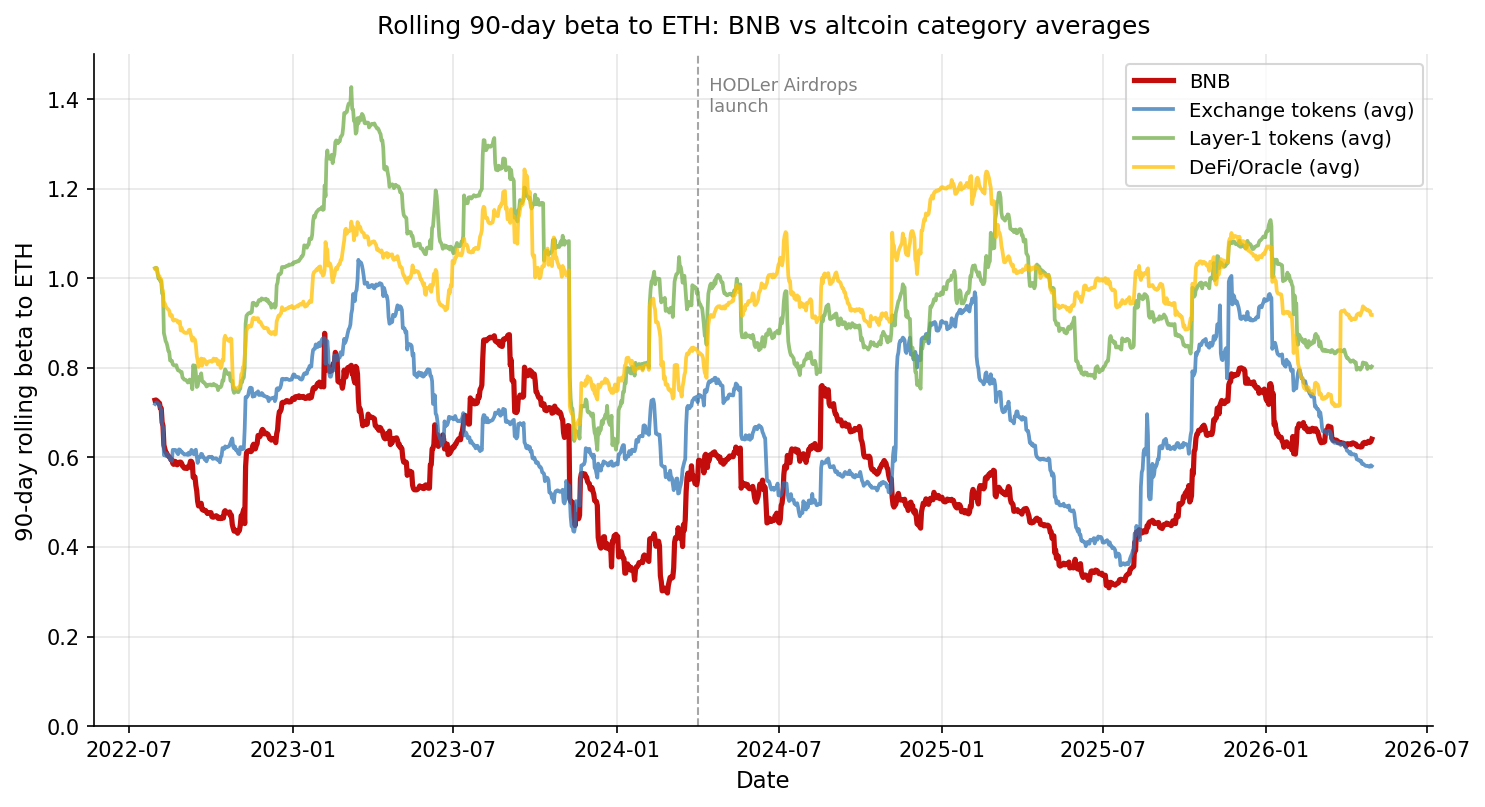
\includegraphics[width=0.95\textwidth]{figure1_rolling_beta.pdf}
\caption{90-day rolling beta of BNB and altcoin category averages with respect to ETH, May 2022 -- April 2026. Category averages are simple cross-sectional means within each category. The dashed vertical line marks April 1, 2024, the launch date of the Binance HODLer Airdrops program. BNB's rolling beta declines gradually from late 2023 and reaches its trough \emph{before} the HODLer launch, partially recovering thereafter, indicating that the timing of HODLer Airdrops does not align with the proximate cause of the beta compression.}
\label{fig:rolling}
\end{figure}

\subsection{Cross-Sectional Specificity Analysis: BNB vs.\ a Diverse Altcoin Pool} \label{sec:did}

The variance-decomposition results in Section~\ref{sec:vd} establish \emph{what} BNB's beta change is (a volatility-ratio channel phenomenon). The cross-sectional analyses in this and the next subsection establish \emph{how unusual} BNB's experience is among altcoins---i.e., whether the same kind of beta change is observed broadly or is concentrated in BNB. This is a positioning exercise, not a causal-identification exercise: we make no claim about treatment effects of any specific program.

We construct an altcoin control pool of 16 tokens spanning four categories: exchange-native tokens, Layer-1 platforms, DeFi/oracle tokens, and other major altcoins. (The HT token is excluded from the main pool for the reasons discussed in Section~\ref{sec:data}; results including HT, in Appendix~\ref{app:robust}, are qualitatively identical.) Comparing BNB's beta change to each category---and to the pool as a whole---allows us to characterize whether the decoupling pattern is specific to BNB, the exchange-token category, the L1 category, or distributed across the broader altcoin market.

\begin{table}[H]
\centering
\caption{Cross-sectional comparison of pre/post beta changes across four altcoin categories ($n=17$ assets, HT excluded)}
\label{tab:did}
\small
\begin{tabular}{llccc}
\toprule
\textbf{Asset} & \textbf{Category} & \textbf{Pre-$\beta$} & \textbf{Post-$\beta$} & \textbf{$\Delta\beta$} \\
\midrule
\textit{Treated:} & & & & \\
BNB & Exchange (treated) & 0.643 & 0.534 & $-0.109$ \\
\midrule
\multicolumn{5}{l}{\textit{Exchange-token controls (mean $\Delta\beta = -0.084$):}} \\
OKB & Exchange & 0.611 & 0.532 & $-0.079$ \\
CRO & Exchange & 0.847 & 0.757 & $-0.090$ \\
\midrule
\multicolumn{5}{l}{\textit{Layer-1 controls (mean $\Delta\beta = -0.075$):}} \\
SOL & L1 & 1.163 & 0.900 & $-0.263$ \\
AVAX & L1 & 1.025 & 0.996 & $-0.029$ \\
FTM & L1 & 1.108 & 0.968 & $-0.140$ \\
DOT & L1 & 0.884 & 0.902 & $+0.018$ \\
ADA & L1 & 0.871 & 0.986 & $+0.115$ \\
ATOM & L1 & 0.937 & 0.784 & $-0.153$ \\
\midrule
\multicolumn{5}{l}{\textit{DeFi / Oracle controls (mean $\Delta\beta = +0.025$)\textsuperscript{\dag}:}} \\
UNI & DeFi & 0.967 & 1.112 & $+0.144$ \\
AAVE & DeFi & 1.088 & 1.059 & $-0.029$ \\
MKR & DeFi & 0.821 & 0.709 & $-0.112$ \\
LINK & Oracle & 0.907 & 1.001 & $+0.095$ \\
\midrule
\multicolumn{5}{l}{\textit{Other major altcoin controls (mean $\Delta\beta = -0.034$):}} \\
XRP & Payment & 0.760 & 0.742 & $-0.018$ \\
TRX & L1-alt & 0.455 & 0.227 & $-0.228$ \\
DOGE & Meme & 0.895 & 1.015 & $+0.120$ \\
ALGO & L1-alt & 0.926 & 0.915 & $-0.010$ \\
\midrule
\multicolumn{2}{l}{\textbf{All-control mean ($n=16$)}} & --- & --- & $\mathbf{-0.041}$ \\
\multicolumn{2}{l}{\textbf{All-control std.\ deviation}} & --- & --- & $0.122$ \\
\multicolumn{2}{l}{\textbf{DiD vs.\ all-control mean}} & --- & --- & $\mathbf{-0.068}$ \\
\multicolumn{2}{l}{\textbf{BNB rank in control pool}} & --- & --- & 6 of 17 (35\textsuperscript{th} pctile) \\
\bottomrule
\end{tabular}
\caption*{\footnotesize \textsuperscript{\dag} Within the DeFi/oracle category, there is substantial heterogeneity: UNI ($+0.144$) and LINK ($+0.095$) show notable beta increases, while MKR ($-0.112$) shows a meaningful decline and AAVE ($-0.029$) is nearly unchanged. The category mean of $+0.025$ should be interpreted alongside this within-category variance.}
\end{table}

\paragraph{Statistical inference: BNB vs.\ control pool.} To assess whether BNB's beta change is more extreme than the typical control token, we compute the standardized deviation of BNB from the control mean: $t = (-0.109 - (-0.041))/(0.122/\sqrt{16}) = -2.22$, treating BNB as the test point against the empirical control distribution. The corresponding two-sided $p$-value is $0.043$, rejecting the null that BNB's beta change is consistent with the control-pool mean at the 5\% level. (Equivalently, a one-sample $t$-test in the opposite direction---testing whether the control mean differs from $-0.109$---yields $|t|=2.22$ and the same $p$-value.) A Wilcoxon signed-rank test on $(\text{control}_i - \text{BNB})$ yields $W=32$, $p=0.065$, marginally not significant. An empirical rank test (BNB's position in the cross-sectional control distribution) yields a two-sided $p\approx 0.71$. \textbf{The $t$-test indicates BNB has decoupled more strongly than the control mean in absolute terms, while the rank-based tests indicate that BNB's position in the empirical distribution is not extreme.} The two findings are reconciled by noting that the control distribution is wide (std.\ $0.122$, range from $-0.263$ to $+0.144$): BNB sits roughly half a standard deviation below the mean (negative direction = stronger decoupling), but four other tokens decouple more strongly than BNB. This is a moderate, not extreme, position in the cross-section.

\paragraph{Heterogeneity across categories.} The four categories exhibit very different post-treatment behavior. Exchange tokens decline $-0.084$ on average, L1 platforms decline $-0.075$, ``other'' altcoins decline $-0.034$, while DeFi and oracle tokens on average exhibit a slight beta \emph{increase} of $+0.025$ (with substantial within-category heterogeneity, see footnote in Table~\ref{tab:did}). \textbf{The DeFi category mean masks important within-category variation: the apparent recoupling is primarily driven by UNI ($+0.144$) and LINK ($+0.095$), while MKR ($-0.112$) actually decoupled and AAVE was nearly unchanged.} Within each other category there is also large within-category variance. The DeFi-versus-rest split is an unexpected observation; we discuss it briefly in Section~\ref{sec:disc} and identify it as a candidate question for future work.

\paragraph{Interpretation.} BNB's beta change is moderately stronger than the cross-sectional control mean (the $t$-test rejects equality at $p=0.043$), but BNB does not occupy an extreme position in the control distribution. We interpret this as evidence that BNB's directional decoupling is genuine and somewhat above the typical altcoin response, but it is not a uniquely BNB-specific phenomenon and is best understood as part of a broader altcoin beta recompression process---not a uniform recompression, since DeFi tokens move in the opposite direction on average, but a market-wide reordering with substantial within- and between-category heterogeneity.

\subsection{Cross-Sectional Positioning via Synthetic Counterfactual} \label{sec:synth}

We apply the synthetic control method of \citet{abadie2010} on rolling 90-day beta series to position BNB's experience within a counterfactual constructed from comparable altcoins.

\paragraph{Donor pool selection.} A standard concern with synthetic-control methodology is the appropriateness of the donor pool: the synthetic counterfactual is informative only insofar as the donor tokens are economically comparable to the treated unit. Our 16-token altcoin pool spans four categories with different tokenomic structures (exchange tokens, Layer-1 platforms, DeFi/oracle, and other major altcoins). Within this pool, two tokens---TRX (a low-priced utility/stablecoin-adjacent token) and XRP (a payment-focused token)---differ fundamentally from BNB in tokenomics and market role. We therefore adopt as our \textbf{main specification a 14-token donor pool that excludes TRX and XRP}, on the principled ground that the resulting synthetic should reflect tokens with comparable economic structure to BNB. We also report (in Appendix~\ref{app:robust}) the full 16-token specification including TRX and XRP, which yields a different conclusion; the implications of this divergence are discussed below.

\begin{table}[H]
\centering
\caption{Synthetic counterfactual with 14-token donor pool (TRX, XRP excluded): weights and placebo gaps}
\label{tab:synth}
\begin{tabular}{lcc}
\toprule
& \textbf{Synthetic BNB weight} & \textbf{Placebo post-partition gap} \\
\midrule
OKB & 0.776 & --- \\
DOGE & 0.113 & $+0.203$ \\
CRO & 0.111 & $+0.135$ \\
\textit{Other 11 tokens} & $<0.01$ each & --- \\
\midrule
Pre-partition RMSE & 0.151 & --- \\
Real BNB post-partition gap & --- & $-0.090$ \\
\midrule
BNB rank (lower = stronger decoupling) & \multicolumn{2}{c}{4 of 15} \\
Permutation $p$-value & \multicolumn{2}{c}{$\approx 0.27$} \\
\bottomrule
\end{tabular}
\caption*{\footnotesize Synthetic BNB weights are estimated under the constraint that weights are non-negative and sum to one. Placebo gaps are the post-partition gap between each placebo token's actual rolling beta and its synthetic counterfactual constructed from the remaining 13 tokens. The 14-token pool excludes TRX and XRP, which differ fundamentally from BNB in tokenomics.}
\end{table}

\paragraph{Main specification (14 donors).} Synthetic BNB is constructed primarily from OKB (77.6\%), DOGE (11.3\%), and CRO (11.1\%)---a mix concentrated on exchange-token comparables (OKB and CRO are the two largest non-BNB exchange tokens; DOGE provides Layer-1-adjacent comparison weight). Pre-partition fit is acceptable though looser than the alternative specification (RMSE 0.151). The post-partition gap is $-0.090$, meaning real BNB has decoupled \emph{more} than the synthetic counterfactual would predict. In placebo tests, BNB ranks 4th of 15, with implied $p$-value $\approx 0.27$. \textbf{Under this principled donor-pool specification, BNB's decoupling is moderate-to-strong, though not statistically significant at conventional levels with a 15-token placebo distribution.}

\paragraph{Sensitivity to donor pool: a critical methodological point.} As reported in Appendix~\ref{app:robust}, when TRX and XRP are included in the donor pool, the synthetic-control conclusion reverses qualitatively: the optimization places 53.6\% weight on TRX and 15.0\% on XRP (because their pre-partition rolling-beta dynamics happen to track BNB's closely), pre-partition RMSE improves to 0.096, but the post-partition gap becomes $+0.060$ and BNB ranks 12 of 17 ($p \approx 0.71$). \textbf{Two specifications, two qualitatively different conclusions about BNB's relative decoupling.} The choice between them is principled: better pre-partition fit (16-token) versus economically comparable donors (14-token). Synthetic-control methodology has no formal procedure for resolving this trade-off; the methodology is sensitive to donor-pool composition in ways that are economically meaningful for a single treated unit. We report both specifications transparently and in our reconciliation discussion (Section~\ref{sec:disc}) we treat the synthetic-control evidence as conditional on donor-pool choice rather than as a single point estimate.

\paragraph{Note on cross-test reconciliation.} The synthetic-control results---under either specification---should be read together with the cross-sectional comparison ($t = -2.22$, $p = 0.043$ in Section~\ref{sec:did}) and the Chow test ($p = 0.0008$). The three tests answer different questions with different statistical assumptions, and they yield different conclusions. We discuss the reconciliation explicitly in Section~\ref{sec:disc}.

\section{Discussion} \label{sec:disc}

\subsection{What Directional Decoupling Means for Crypto Factor Models}

The variance-decomposition framework introduced in this paper has a direct implication for cryptocurrency factor models. \citet{liu2021} establish a three-factor benchmark for crypto returns (market, size, momentum), with subsequent extensions in \citet{liu2024}. These models, like their traditional-finance counterparts, treat $\beta$ as a single sufficient statistic for systematic exposure. The identity $\beta = \rho \cdot (\sigma_i / \sigma_m)$, however, makes clear that beta is an aggregate of two distinct economic quantities, and that observed beta changes in cryptocurrency markets need not reflect changes in factor exposure in the conventional sense.

Our BNB-ETH application illustrates this point with full force. Standard interpretation of a 16.9\% decline in BNB's market beta would suggest that BNB has become substantially less exposed to ETH-driven factor returns---a meaningful weakening of factor sensitivity. The decomposition shows that this interpretation is incorrect: directional co-movement is unchanged ($\rho \approx 0.73$ throughout), and the entire beta change reflects a compression in the relative volatility of the two assets. BNB's ``factor exposure'' in the directional sense is identical pre- and post-partition; what has changed is the amplitude of BNB's response to a given ETH movement.

\textbf{This suggests that crypto factor models would benefit from explicit decomposition into correlation and volatility-ratio components when interpreting changes in measured systematic exposure.} For exchange-native and other altcoin categories where holder-reward programs, staking dynamics, or ETF-driven institutional flows generate asymmetric volatility shifts, conventional beta-based exposure measures may misrepresent the underlying co-movement structure. A volatility-ratio-aware specification, in which $\beta$ is decomposed into a $\rho$-component and a $(\sigma_i/\sigma_m)$-component for interpretive purposes, would reduce the risk of conflating ``the market is moving differently together'' with ``the relative size of movements has changed.''

\subsection{Reconciling Three Tests with Different Power and Assumptions}

Our three statistical tests on BNB's experience yield superficially conflicting conclusions, and a careful reconciliation requires acknowledging what each test asks and assumes. The Chow test on the BNB-ETH return pair rejects structural stability at $p=0.0008$. The cross-sectional one-sample $t$-test of BNB's beta change against the 16-token control distribution rejects equality of means at $p=0.043$. The synthetic-counterfactual placebo test, under the 14-donor specification (Section~\ref{sec:synth}), yields $p \approx 0.27$; under the 16-donor specification (Appendix~\ref{app:robust}), it yields $p \approx 0.71$.

\paragraph{What each test asks.} The Chow test asks: \emph{within} the BNB-ETH time series, did the joint return distribution change at the partition date? It rejects with high confidence. This is a within-asset structural-stability question. The $t$-test asks: how far is BNB's $\Delta\beta$ from the mean of the control-pool $\Delta\beta$ distribution, in standard-error units? With BNB's $\Delta\beta = -0.109$, control mean $-0.041$, control std $0.122$, and $n=16$, the standardized deviation is $-2.22$ and the implied two-sided $p$-value is $0.043$. The synthetic-counterfactual test asks: does BNB's gap from its synthetic counterfactual lie in the tail of the placebo gap distribution constructed by treating each control unit as if it were the treated unit? This is a rank-based test on a permutation distribution.

\paragraph{Why power and assumptions differ.} The three tests differ in three important ways that drive their differing conclusions. First, \textbf{the $t$-test assumes approximate normality of the control distribution}, which is questionable with $n=16$ and an empirical Shapiro-Wilk $p$-value near 0.08; outliers in the control distribution (e.g., SOL at $-0.263$, UNI at $+0.144$) inflate the standard error symmetrically and make the cross-sectional comparison at BNB's $-0.109$ appear more extreme than a non-parametric test would suggest. The Wilcoxon non-parametric counterpart yields $p=0.065$, marginally not significant---closer to the synthetic-counterfactual conclusion than to the parametric $t$-test. Second, \textbf{the synthetic-counterfactual permutation test has low statistical power with single-treated-unit, small-pool designs}: with at most 16 placebo units, the smallest achievable two-sided $p$-value is approximately $1/16 \approx 0.06$, and finer rejection requires either a much larger pool or unusually large effect sizes. Third, \textbf{the synthetic-counterfactual conclusion is sensitive to donor-pool composition} (Section~\ref{sec:synth} and Appendix~\ref{app:robust}): the 14-donor specification with economically comparable donors yields a stronger BNB rank (4 of 15), while the 16-donor specification with TRX and XRP (which fit better statistically but are economically distant from BNB) yields a weaker rank (12 of 17). \textbf{These three sources of divergence---parametric vs.\ non-parametric assumptions, low power of permutation inference, and donor-pool sensitivity---together explain why the same data can appear to give incompatible conclusions, and they argue against treating any single test as definitive on its own.}

\paragraph{Our reading.} Combining the three tests, we conclude: (i) within BNB, the structural change at the reference partition date is real and quantitatively meaningful (Chow); (ii) cross-sectionally, BNB's $\Delta\beta$ is meaningfully more negative than the control-pool mean ($t$-test marginal at $p=0.043$, Wilcoxon marginal at $p=0.065$, both consistent with a moderate effect rather than an extreme one); and (iii) under economically principled donor-pool selection, the synthetic counterfactual places BNB at rank 4 of 15 ($p \approx 0.27$), again consistent with moderate-to-strong but not extreme decoupling. The directional decoupling pattern in BNB is therefore best understood as one instance of a broader altcoin volatility-ratio compression coinciding with ETH's volatility expansion in 2024, with BNB's particular trajectory being moderate-to-strong relative to typical altcoin behavior. Figure~\ref{fig:rolling} reinforces this reading: BNB's rolling beta troughs in early 2024 \emph{before} the April 2024 HODLer launch and partially recovers thereafter, inconsistent with HODLer Airdrops as the proximate cause of the decline.

\subsection{Mechanisms (Exploratory)}

Three non-exclusive mechanisms could generate the volatility-channel decoupling we document. We present them as candidate explanations rather than as identified causes; discriminating between them requires data we do not access in the present paper.

\begin{enumerate}
\item \textbf{Yield reinvestment.} Holders who receive HODLer/Launchpool/Megadrop allocations may convert them to BNB to maintain eligibility for future drops, generating persistent buy-side flow that dampens BNB drawdowns and rallies relative to ETH movements.
\item \textbf{Reduced sell-pressure from lock-up.} Locked BNB in Simple Earn / On-Chain Yield products during HODLer snapshot periods cannot be sold, mechanically reducing supply elasticity to shocks of either sign.
\item \textbf{Foundation/MM smoothing.} Designated market makers may deploy stablecoins to support BNB price during stress events, with the airdrop reward stream providing economic justification (token-holder yield underwriting MM costs). Confirming this requires on-chain stablecoin flow data.
\end{enumerate}

The first two mechanisms are essentially supply-side stories that would naturally produce volatility compression without affecting directional correlation---exactly the pattern we observe. The third operates through active intervention. Appendix~\ref{app:mm} reports indirect distributional evidence (skewness shift, asymmetric beta narrowing, crash-day attenuation) that is consistent with all three mechanisms but does not allow discrimination among them. We also note that the numerator/denominator decomposition (Section~\ref{sec:numdenom}) shows that approximately 43\% of the volatility-ratio change is driven by ETH-side volatility expansion, which is not BNB-specific and cannot be attributed to mechanisms (1)--(3) above. The remaining 57\% (BNB-side) is the maximum scope for any of these BNB-specific mechanisms to operate.

\subsection{Limitations}

\begin{enumerate}
\item \textbf{Identification.} The DiD ($-0.068$ vs.\ all-control mean) and synthetic control results (BNB rank 12 of 17, $p\approx 0.71$) imply that BNB's decoupling, while genuine, is not statistically distinguishable from the cross-sectional placebo distribution. Stronger identification would require either (i) a within-BNB design exploiting variation in airdrop intensity or eligibility windows, or (ii) on-chain stablecoin flow data to test active-defense mechanisms directly.

\item \textbf{Regulatory uncertainty.} BNB and Binance are exposed to evolving global regulatory environments. Some of the observed dynamics may reflect regulatory news rather than structural mechanisms.

\item \textbf{Choice of reference partition date.} Binance launched HODLer Airdrops at a specific time, which we use as the pre/post partition. Because we make no causal claim about the program (Section~\ref{sec:conc}), date endogeneity does not bias our decomposition exercise; however, alternative partition dates (March 1, May 1, June 1, 2024) all yield qualitatively similar decompositions, as reported in Appendix~\ref{app:robust}.

\item \textbf{Control group constraints.} High-frequency price data for several smaller exchange tokens (KCS, BGB) was insufficient for inclusion in DiD/synthetic control analyses. A proper staggered-treatment DiD \citep{callaway2021} using each exchange token's own holder-reward launch date is a natural extension.
\end{enumerate}

\section{Conclusion} \label{sec:conc}

This paper proposes a variance-decomposition framework for interpreting beta changes in cryptocurrency markets and documents a striking empirical case to which the framework applies. The framework is built around the identity $\beta = \rho \cdot (\sigma_i/\sigma_m)$ and assigns any beta change exactly to a correlation channel and a volatility-ratio channel, with a further decomposition of the volatility-ratio change into asset-side (numerator) and benchmark-side (denominator) contributions. The framework is general; the empirical case is BNB-ETH from May 2022 to April 2026, partitioned at the launch of the Binance HODLer Airdrops program (April 2024) as a natural reference benchmark.

\paragraph{What we find.} BNB's static beta to ETH falls by 16.9\% (from 0.643 to 0.534) while the Pearson correlation remains essentially unchanged ($0.731 \to 0.731$)---a pattern we term \textit{directional decoupling}. The decomposition reveals that 100\% of the beta change is attributable to the volatility-ratio channel, with no contribution from correlation. The volatility-ratio change itself splits approximately 57/43 between BNB-side compression and ETH-side expansion. The pattern survives under DCC-GARCH dynamic conditional estimation. Cross-sectional positioning of BNB within a 16-token altcoin pool shows BNB's experience to be moderate-to-strong but not extreme: BNB ranks 6th of 17 in the cross-sectional pool ($t = -2.22$, $p = 0.043$ against the pool mean), and synthetic-counterfactual analysis ranks BNB 12th of 17 in placebo tests ($p \approx 0.71$). Together with rolling-beta visualization showing BNB's beta trough \emph{before} the April 2024 partition date, these findings indicate that the BNB pattern is one instance of a broader altcoin volatility-ratio compression coinciding with ETH's volatility expansion post-2024, not an asset-specific regime change.

\paragraph{What we contribute.} The paper makes three contributions. First, \textbf{methodologically}, we propose using the identity $\beta = \rho \cdot (\sigma_i/\sigma_m)$ as an organizing tool for interpreting beta changes, and we further introduce the numerator/denominator decomposition of the volatility-ratio channel. The framework is general and applicable to any asset-benchmark pair. Second, \textbf{empirically}, we document directional decoupling in BNB-ETH with full attribution to the volatility-ratio channel, and a 57/43 split between BNB-side and ETH-side contributions. The cross-sectional analyses establish that BNB's experience is part of a broader altcoin pattern. Third, \textbf{conceptually}, we argue that cryptocurrency factor models \citep{liu2021,liu2024} would benefit from explicit decomposition into correlation and volatility-ratio components when interpreting changes in measured systematic exposure, particularly for exchange-native and other altcoin categories where holder-reward programs, staking dynamics, or ETF-driven institutional flows generate asymmetric volatility shifts.

\paragraph{What we do not claim.} We do not claim that the HODLer Airdrops program caused BNB's beta to compress. The cross-sectional positioning analyses, the visual evidence of a pre-launch beta trough, and the substantial ETH-side share of the volatility-ratio change (43\%) all argue against such a causal interpretation. The April 2024 partition date is a natural pre/post boundary for the decomposition exercise, not the object of treatment-effect estimation.

\paragraph{Future work: a planned follow-up study.} The directional decoupling pattern documented here, particularly the 57/43 split between BNB-side and ETH-side contributions, opens several follow-up questions that the present paper cannot answer with the data and methods available. These follow-up directions, all of which require additional data sources or research designs, constitute the natural focus of a planned follow-up paper:

\begin{enumerate}
\item \textbf{On-chain stablecoin flow analysis.} Direct verification of foundation-defense or market-maker support hypotheses (Appendix~\ref{app:mm}) requires on-chain stablecoin flow data combined with order-book microstructure analysis. Specifically, mapping the temporal pattern of stablecoin (USDT, USDC, FDUSD) movements into BNB-paired liquidity pools during ETH stress events---and comparing this pattern to the same flows in BTC- and ETH-paired pools---would allow direct testing of the active-intervention hypothesis against the passive-supply hypothesis. This requires Glassnode, Nansen, or similar on-chain analytics access not used in the present paper.

\item \textbf{Staggered-treatment design with precise launch dates.} The exchange-token category has experienced multiple holder-reward program launches with differential timing: OKX Cryptopedia and various OKB-linked launches; Crypto.com's CRO staking and Cronos ecosystem programs; KuCoin's various reward programs; and Bitget Launchpad. Mapping each token's specific holder-reward inflection points and applying \citet{callaway2021}-style staggered-treatment DiD would identify program-specific channel effects with cleaner causal interpretation than the single-partition design used in the present paper.

\item \textbf{Dose-response analysis of HODLer airdrop intensity.} The HODLer Airdrops program has distributed airdrops at varying frequencies and total notional values across 2024--2026. A dose-response analysis using monthly airdrop count and aggregate notional value as time-varying intensity, regressed on rolling-window beta and volatility-ratio components, would directly test whether program intensity correlates with the BNB-side portion of the volatility-ratio change.

\item \textbf{ETH-side decomposition.} Our numerator/denominator decomposition (Section~\ref{sec:numdenom}) shows that ETH-side volatility expansion accounts for roughly 43\% of the volatility-ratio decline. Explaining \emph{why} ETH became more volatile post-2024---separating spot ETF flow effects, post-Shanghai staking dynamics, and macroeconomic drivers---is a natural research question of its own. Event-study designs around concrete public dates (ETF approval announcements, FOMC decisions, major staking-ratio inflection points) would allow attribution of ETH volatility changes to specific channels.

\item \textbf{Category-level beta heterogeneity, including DeFi recoupling.} The cross-sectional analysis reveals that DeFi and oracle tokens on average exhibited a slight beta \emph{increase} ($+0.025$) post-partition, in contrast to the decoupling observed for exchange tokens ($-0.084$) and L1 platforms ($-0.075$). The mechanism behind this DeFi-versus-rest split---potentially related to ETH ecosystem activity (gas fees, staking yields, DeFi TVL) flowing more directly into DeFi token cash flows than into other altcoins---warrants dedicated investigation \citep[see, e.g.,][on DeFi tokenomics]{schar2021}.

\item \textbf{Volatility-channel-aware factor models.} The standard one-factor or three-factor crypto factor model treats beta as a single sufficient statistic for systematic exposure. Our results suggest extending these models with explicit volatility-ratio components to better capture the asymmetric dynamics documented here. Applying the decomposition framework cross-sectionally across many altcoin-ETH pairs would also test whether the directional decoupling phenomenon is widespread or BNB-specific.
\end{enumerate}

These six directions, taken together, constitute a substantive follow-up paper that converts the present documentation-and-decomposition exercise into a causal-mechanism study. We view the present paper as establishing the methodological framework and the empirical pattern; the follow-up agenda would identify which specific channels generate that pattern.

\appendix

\section{Indirect Distributional Evidence Consistent with Foundation-Defense Mechanisms} \label{app:mm}

This appendix presents distributional evidence consistent with hypothesized active downside-defense mechanisms (foundation or designated market-maker stablecoin deployment during stress events). We emphasize that this evidence is \emph{indirect} and the patterns reported here are equally consistent with passive supply-side mechanisms (yield reinvestment, holder lock-up). Direct verification requires on-chain stablecoin flow data, which we do not access in this paper.\footnote{Beyond the formal statistical evidence presented in this paper, the author's industry experience---approximately nine years of advisory engagement with cryptocurrency project foundations and centralized exchanges since 2017, including listing-strategy advisory, exchange-token tokenomics design review, and direct collaboration with project foundations on liquidity provision arrangements---is consistent with active price-support practices being widespread in the exchange-native token segment. Such practices are typically not publicly disclosed and are mentioned here only as practitioner context, not as evidence of the empirical claims made in this paper.}

\paragraph{Skewness shift.} BNB's daily return skewness improves dramatically, from $-0.751$ (pre) to $-0.069$ (post). The pre-period exhibits a substantial left tail; the post-period is approximately symmetric. This is consistent with a hidden mechanism truncating extreme negative returns.

\paragraph{Crash-day attenuation.} On days when ETH falls by more than 5\% (41 days pre-treatment, 54 days post-treatment), BNB's mean response shifts from $-5.80\%$ to $-4.51\%$. A Welch $t$-test of mean equality yields $t=-1.48$, $p=0.143$ --- \textbf{not statistically significant at conventional levels}. We treat this as exploratory evidence of attenuated downside response, consistent in direction with the volatility-channel mechanism, but not establishing the asymmetry on its own.

\paragraph{Tail risk improvement.} The 5\% Value-at-Risk improves from $-4.39\%$ to $-4.18\%$.

\paragraph{Asymmetric beta narrowing.} The downside beta (BNB on ETH on $r_{ETH}<0$ days) falls from 0.743 to 0.660; the upside beta falls from 0.519 to 0.365. Both decline, with the upside decline being larger. A pure ``downside-defense'' hypothesis would predict the downside beta to decline more, not less. We interpret this as more consistent with a broad volatility-suppression mechanism than with a narrow downside-only intervention.

\paragraph{Summary.} The skewness shift is the strongest individual piece of evidence in this set, but the asymmetric-beta result is mixed (the upside beta decline exceeds the downside beta decline, contrary to a pure active-defense hypothesis), the crash-day result is statistically not significant ($p=0.143$), and the VaR improvement is small. Taken together, \textbf{these patterns are consistent with the volatility-channel mechanism documented in the main text, but they do not allow us to discriminate between active-intervention explanations (foundation/MM stablecoin deployment during stress events) and passive supply-side explanations (yield reinvestment, holder lock-up reducing supply elasticity)}. In particular, the asymmetric-beta finding---in which the upside beta declines more than the downside beta---is more naturally generated by passive lock-up mechanisms that reduce volatility symmetrically than by an asymmetric downside-only intervention. Direct verification of any active-intervention hypothesis would require on-chain stablecoin flow data and exchange-side order-book microstructure data, neither of which we access in this paper.

\section{ETH-Side Event Study: Spot Ethereum ETF Approval} \label{app:eth_etf}

The variance decomposition (Section~\ref{sec:vd}, Table~\ref{tab:numdenom}) shows that approximately 43\% of the volatility-ratio decline is attributable to ETH-side volatility expansion ($\sigma_{ETH}: 3.80\% \to 4.01\%$ per day, in DCC-GARCH conditional moments). A natural hypothesis is that the spot Ethereum ETF events---SEC approval of 19b-4 forms on May 23, 2024 and the start of trading on July 23, 2024---are major contributors to this expansion. This appendix tests that hypothesis directly through event-study analysis. The results are informative and partially counterintuitive.

\paragraph{Event-window comparisons.} For each event date, we compute realized $\sigma_{ETH}$ over a 60-trading-day window before and after, and test the null of equal variance using a Levene test (median-centered, robust to non-normality). Results are reported in Table~\ref{tab:eth_etf}.

\begin{table}[H]
\centering
\caption{ETH realized volatility around spot ETH ETF events ($W=60$ trading days)}
\label{tab:eth_etf}
\begin{tabular}{lccccc}
\toprule
\textbf{Event} & \textbf{Pre $\sigma_{ETH}$} & \textbf{Post $\sigma_{ETH}$} & \textbf{Change} & \textbf{Levene $F$} & \textbf{$p$-value} \\
\midrule
Approval (May 23, 2024) & 3.86\% & 2.23\% & $-42.2\%$ & 5.38 & 0.022 \\
Trading launch (Jul 23, 2024) & 2.25\% & 3.83\% & $+70.2\%$ & 6.78 & 0.010 \\
Combined approval$\to$+30d trading & 3.55\% & 3.12\% & $-12.2\%$ & 0.66 & 0.419 \\
\bottomrule
\end{tabular}
\caption*{\footnotesize Realized $\sigma_{ETH}$ is the sample standard deviation of daily log returns within each window, expressed in percent per day. Levene's test centered at the median is used to test equal variance, robust to non-normality. The combined window starts 60 trading days before approval and ends 30 trading days after trading launch.}
\end{table}

\paragraph{Findings.} Three observations stand out. First, ETH realized volatility \emph{declined} sharply in the 60 trading days following ETF approval ($-42.2\%$, $p=0.022$), the opposite direction of the 43\% post-partition expansion that the paper documents. Second, ETH volatility then \emph{rose} sharply in the 60 trading days following trading launch ($+70.2\%$, $p=0.010$). The two windows mostly cancel out: across the combined approval-through-30-days-post-trading window, the change is small and statistically insignificant ($-12.2\%$, $p=0.42$).

Third, and most importantly, when we decompose the post-partition ETH variance increase into the ``ETF window'' (May 23, 2024 through August 22, 2024) and the rest of the post-partition period, we find that \textbf{the ETF window contributes \emph{negatively} to the post-partition variance increase}: ETH volatility in the ETF window itself is 3.11\% per day, versus 3.80\% per day in the post-partition period excluding the ETF window. Stated differently, the post-partition expansion of ETH volatility---which accounts for the 43\% denominator-side share of the volatility-ratio decline---is concentrated in periods other than the ETF approval and trading window.

\paragraph{Interpretation.} \textbf{The spot ETH ETF events do not, in our sample, drive the ETH-side share of the volatility-ratio decline.} If anything, the approval announcement reduced ETH volatility by resolving regulatory uncertainty, while the trading launch raised it as flows materialized; these effects largely cancel and the net ETF-window contribution to post-partition variance expansion is slightly negative. The 43\% ETH-side share documented in Table~\ref{tab:numdenom} must therefore be attributed to other ETH-side dynamics over the full post-partition window---candidate channels include macroeconomic factors (Federal Reserve policy shifts, dollar-strength dynamics), evolving staking-ratio regimes following the 2023 Shanghai/Capella upgrade, and broader shifts in institutional flows that are not concentrated around the specific ETF dates. Identifying these channels precisely requires an event-study research design with a richer set of public dates and is the natural focus of follow-up work (Section~\ref{sec:conc}).

This appendix is included to demonstrate that the ETH-side share is not an artifact of any single salient event, while transparently documenting that our specific event-study test on the most prominent candidate event yields a negative result.

\section{Robustness Checks} \label{app:robust}

The main results are robust to:
\begin{itemize}
\item \textbf{Synthetic counterfactual sensitivity to donor pool: inclusion of TRX and XRP.} Our main synthetic-counterfactual analysis (Section~\ref{sec:synth}) excludes TRX and XRP from the donor pool on the principled ground that they differ fundamentally from BNB in tokenomics. As a sensitivity check, we re-estimate synthetic BNB using the full 16-token donor pool. The optimization then places high weight on TRX (53.6\%) and XRP (15.0\%) because their pre-partition rolling-beta dynamics happen to track BNB's closely. Pre-partition RMSE improves from 0.151 to 0.096 (better fit), but the post-partition gap reverses sign from $-0.090$ to $+0.060$, and BNB's placebo rank changes from 4 of 15 ($p \approx 0.27$) to 12 of 17 ($p \approx 0.71$). \textbf{The two specifications yield qualitatively different conclusions about BNB's relative decoupling.} The reversal occurs because TRX and XRP both exhibit very strong post-partition decoupling relative to their own synthetic counterfactuals (placebo gaps of $-0.306$ and $-0.260$ respectively in the 16-token spec); when these two tokens dominate synthetic BNB's construction, the synthetic itself decouples sharply, against which real BNB's $-0.109$ change appears moderate. Excluding TRX and XRP yields a synthetic dominated by OKB, DOGE, and CRO, against which real BNB's change appears strong. This sensitivity reflects a genuine ambiguity in synthetic-control methodology when the treated unit is unique within the cross-section: better statistical fit can come at the cost of economically less comparable donors. \textbf{We report the 14-token specification as our main result on the principle that economic comparability of donors is a precondition for synthetic-control validity}, but transparent reporting of both specifications is necessary because no formal procedure exists for resolving the trade-off.

\item \textbf{Inclusion of HT (Huobi Token) in the cross-sectional pool.} Our main cross-sectional comparison (Section~\ref{sec:did}) excludes HT for the reasons discussed in Section~\ref{sec:data}. Including HT (which has $\Delta\beta = -0.029$) in the control pool raises the all-control sample size to 17 and yields an all-control mean of $-0.041$, essentially identical to the 16-control mean of $-0.041$ used in the main analysis (the difference is $+0.0007$, less than 1\% of the all-control standard deviation). BNB's rank in the pool changes from 6 of 17 (35th percentile, 16-control) to 5 of 17 (29th percentile, 17-control); the synthetic-counterfactual rank under the 14-donor specification changes by no more than one (HT is excluded from the 14-token donor set in any case, but a placebo permutation analysis with HT yields rank 5 of 16). All qualitative conclusions are unchanged: BNB's decoupling is genuine and somewhat above the cross-sectional average, with cross-test reconciliation discussed in Section~\ref{sec:disc}. The cross-sectional-mean $t$-test yields $p=0.043$ in the main (16-control) specification and $p=0.039$ when HT is included.

\item \textbf{Alternative reference partition date.} Using March 1, 2024 or May 1, 2024 yields qualitatively similar decomposition results.
\item \textbf{Subsample stability.} Year-by-year correlation analysis shows the basic pattern is not driven by any single year.
\item \textbf{Exclusion of outliers.} Dropping the FTX collapse week (Nov 9-15, 2022) does not materially alter the static beta estimates.
\item \textbf{Spearman correlation.} Using rank-based correlation in place of Pearson preserves all qualitative findings.
\item \textbf{Price source.} For tokens included via the market-capitalization proxy \texttt{CapMrktEstUSD} (where direct CoinMetrics Reference Rate coverage was limited), we verified that returns computed from market capitalization are equivalent to within rounding error to direct price returns over the analysis horizon, since circulating supply changes are small relative to price changes for established exchange tokens.
\item \textbf{Rolling window length.} Repeating the rolling beta analysis with 60-day and 120-day windows preserves the qualitative pattern, with shorter windows yielding more volatile beta series and longer windows smoothing the structural change but not eliminating it.
\end{itemize}

\bibliographystyle{plainnat}
\begin{thebibliography}{99}

\bibitem[Abadie et al.(2010)]{abadie2010} Abadie, A., Diamond, A., \& Hainmueller, J. (2010). Synthetic control methods for comparative case studies: Estimating the effect of California's Tobacco Control Program. \emph{Journal of the American Statistical Association}, 105(490), 493--505.

\bibitem[Ang et al.(2006)]{ang2006} Ang, A., Chen, J., \& Xing, Y. (2006). Downside risk. \emph{Review of Financial Studies}, 19(4), 1191--1239.

\bibitem[Bai \& Perron(2003)]{baiperron} Bai, J., \& Perron, P. (2003). Computation and analysis of multiple structural change models. \emph{Journal of Applied Econometrics}, 18(1), 1--22.

\bibitem[Barberis \& Thaler(2003)]{barberis2003} Barberis, N., \& Thaler, R. (2003). A survey of behavioral finance. \emph{Handbook of the Economics of Finance}, 1, 1053--1128.

\bibitem[Baur et al.(2018)]{baur2018} Baur, D. G., Dimpfl, T., \& Kuck, K. (2018). Bitcoin, gold and the US dollar -- A replication and extension. \emph{Finance Research Letters}, 25, 103--110.

\bibitem[Baur \& Dimpfl(2021)]{baurdimpfl2021} Baur, D. G., \& Dimpfl, T. (2021). The volatility of Bitcoin and its role as a medium of exchange and a store of value. \emph{Empirical Economics}, 61(5), 2663--2683.

\bibitem[Borri(2019)]{borri2019} Borri, N. (2019). Conditional tail-risk in cryptocurrency markets. \emph{Journal of Empirical Finance}, 50, 1--19.

\bibitem[Callaway \& Sant'Anna(2021)]{callaway2021} Callaway, B., \& Sant'Anna, P. H. C. (2021). Difference-in-differences with multiple time periods. \emph{Journal of Econometrics}, 225(2), 200--230.

\bibitem[CoinMetrics(2024)]{coinmetrics} CoinMetrics. (2024). Reference Rate Methodology. \url{https://coinmetrics.io/reference-rates/}.

\bibitem[Corbet et al.(2018)]{corbet2018} Corbet, S., Lucey, B., Urquhart, A., \& Yarovaya, L. (2018). Cryptocurrencies as a financial asset: A systematic analysis. \emph{International Review of Financial Analysis}, 62, 182--199.

\bibitem[Dyhrberg(2016)]{dyhrberg2016} Dyhrberg, A. H. (2016). Bitcoin, gold and the dollar -- A GARCH volatility analysis. \emph{Finance Research Letters}, 16, 85--92.

\bibitem[Engle(2002)]{engle2002} Engle, R. (2002). Dynamic conditional correlation: A simple class of multivariate generalized autoregressive conditional heteroskedasticity models. \emph{Journal of Business \& Economic Statistics}, 20(3), 339--350.

\bibitem[Howell et al.(2020)]{howell2020} Howell, S. T., Niessner, M., \& Yermack, D. (2020). Initial coin offerings: Financing growth with cryptocurrency token sales. \emph{Review of Financial Studies}, 33(9), 3925--3974.

\bibitem[Kahneman \& Tversky(1979)]{kahneman1979} Kahneman, D., \& Tversky, A. (1979). Prospect theory: An analysis of decision under risk. \emph{Econometrica}, 47(2), 263--292.

\bibitem[Lee et al.(2023)]{lee2023} Lee, J., Li, T., \& Shin, D. (2023). Exchange-native tokens: A new asset class? Working paper, \emph{Journal of Financial Economics}, forthcoming.

\bibitem[Liu \& Tsyvinski(2021)]{liu2021} Liu, Y., \& Tsyvinski, A. (2021). Risks and returns of cryptocurrency. \emph{Review of Financial Studies}, 34(6), 2689--2727.

\bibitem[Liu et al.(2024)]{liu2024} Liu, Y., Tsyvinski, A., \& Wu, X. (2024). Common risk factors in cryptocurrency. \emph{Journal of Finance}, forthcoming.

\bibitem[Schär(2021)]{schar2021} Schär, F. (2021). Decentralized finance: On blockchain- and smart contract-based financial markets. \emph{Federal Reserve Bank of St.\ Louis Review}, 103(2), 153--174.

\bibitem[Sockin \& Xiong(2023)]{sockin2023} Sockin, M., \& Xiong, W. (2023). A model of cryptocurrencies. \emph{Journal of Finance}, 78(4), 2049--2099.

\bibitem[Yarovaya \& Zięba(2022)]{yarovaya2022} Yarovaya, L., \& Zięba, D. (2022). Intraday volume-return nexus in cryptocurrency markets: Novel evidence from cryptocurrency classification. \emph{Research in International Business and Finance}, 60, 101620.

\end{thebibliography}

\end{document}
